% $Header: /cvsroot/latex-beamer/latex-beamer/solutions/conference-talks/conference-ornate-20min.en.tex,v 1.6 2004/10/07 20:53:08 tantau Exp $

\documentclass{beamer}
%\documentclass[handout]{beamer}
%\usepackage{pgfpages}
%\pgfpagesuselayout{2 on 1}[a4paper,border shrink=5mm]

% This file is a solution template for:

% - Talk at a conference/colloquium.
% - Talk length is about 20min.
% - Style is ornate.



% Copyright 2004 by Till Tantau <tantau@users.sourceforge.net>.
%
% In principle, this file can be redistributed and/or modified under
% the terms of the GNU Public License, version 2.
%
% However, this file is supposed to be a template to be modified
% for your own needs. For this reason, if you use this file as a
% template and not specifically distribute it as part of a another
% package/program, I grant the extra permission to freely copy and
% modify this file as you see fit and even to delete this copyright
% notice.


\mode<presentation>
{
%  \usetheme{Warsaw}
%  \usetheme{Boadilla}
%  \usetheme{Goettingen}
%  \usetheme{Hannover}
%  \usetheme{Madrid}
%  \usetheme{Marburg}
%  \usetheme{Montpellier}
%  \usetheme{Pittsburgh}
  \usetheme{Hawke}
  % or ...

  \setbeamercovered{transparent}
  % or whatever (possibly just delete it)
}


\usepackage[english]{babel}
% or whatever

\usepackage[latin1]{inputenc}
% or whatever

\usepackage{times}
\usepackage[T1]{fontenc}
% Or whatever. Note that the encoding and the font should match. If T1
% does not look nice, try deleting the line with the fontenc.

\usepackage{multimedia}


%%%%%%
% My Commands
%%%%%%

\newcommand{\ml}{{\sc matlab}}
\newcommand{\bb}{{\boldsymbol{b}}}
\newcommand{\bx}{{\boldsymbol{x}}}
\newcommand{\by}{{\boldsymbol{y}}}
\newcommand{\bfm}[1]{{\boldsymbol{#1}}}

%%%%

\title[Lecture 18] % (optional, use only with long paper titles)
{Lecture 18 - Runge-Kutta and Multistep Methods}

% \subtitle
% {Include Only If Paper Has a Subtitle}

\author[I. Hawke] % (optional, use only with lots of authors)
{I.~Hawke}
% - Give the names in the same order as the appear in the paper.
% - Use the \inst{?} command only if the authors have different
%   affiliation.

\institute[University of Southampton] % (optional, but mostly needed)
{
%  \inst{1}%
  School of Mathematics, \\
  University of Southampton, UK
}
% - Use the \inst command only if there are several affiliations.
% - Keep it simple, no one is interested in your street address.

\date[Semester 1] % (optional, should be abbreviation of conference name)
{MATH3018/6141, Semester 1}
% - Either use conference name or its abbreviation.
% - Not really informative to the audience, more for people (including
%   yourself) who are reading the slides online

\subject{Numerical methods}
% This is only inserted into the PDF information catalog. Can be left
% out.



% If you have a file called "university-logo-filename.xxx", where xxx
% is a graphic format that can be processed by latex or pdflatex,
% resp., then you can add a logo as follows:

\pgfdeclareimage[height=0.5cm]{university-logo}{mathematics_7469}
\logo{\pgfuseimage{university-logo}}



% Delete this, if you do not want the table of contents to pop up at
% the beginning of each subsection:
%  \AtBeginSubsection[]
%  {
%    \begin{frame}<beamer>
%      \frametitle{Outline}
%      \tableofcontents[currentsection,currentsubsection]
%    \end{frame}
%  }
\AtBeginSection[]
{
  \begin{frame}<beamer>
    \frametitle{Outline}
    \tableofcontents[currentsection]
  \end{frame}
}


% If you wish to uncover everything in a step-wise fashion, uncomment
% the following command:

%\beamerdefaultoverlayspecification{<+->}


\begin{document}

\begin{frame}
  \titlepage
\end{frame}

\section{Runge-Kutta methods}

\subsection{Runge-Kutta methods}

\begin{frame}
  \frametitle{Runge-Kutta methods for IVPs}

  Considering IVPs of the form
  \begin{equation*}
    \by'(x) = \bfm{f}(x, \by(x)).
  \end{equation*}

  We looked at multistage (e.g.\ Runge-Kutta) methods. These
  \begin{itemize}
  \item self start,
  \item  compute next iteration by combining estimates of $\bfm{f}$ to
    improve order of accuracy.
  \end{itemize} \pause

  \vspace{1ex}

  Methods constructed by matching terms in Taylor expansion; ensures
  local truncation error is a certain order. May improve efficiency by
  checking if results are ``good enough'' at given $h$.

\end{frame}

\begin{frame}
  \frametitle{Comparing errors}

  Use $y_e(x_0 + h)$ as the \emph{exact} solution to
  \begin{equation*}
    y'(x) = f(x, y(x)), \quad y(x_0) = y_0.
  \end{equation*}
  Consider numerical solution $y_h(x_0 + h)$ for one step (many
  stages) of a multistage method. \pause By construction the Taylor
  expansion implies
  \begin{equation*}
    | y_e(x_0 + h) - y_h(x_0 + h) | = C h^{s+1}.
  \end{equation*} \pause

  \begin{overlayarea}{\textwidth}{0.4\textheight}
    \only<3-4|handout:1>
    {
      Know that method has order $s$; to compute error also
      need $C$.
    }
    \only<4|handout:1>
    {

      \vspace{1ex}
      Can use Richardson extrapolation variant: compare the error with
      two different step sizes.
    }
    \only<5-6|handout:2>
    {
      By assumption taking two steps of size $h/2$ gives
      \begin{equation*}
        | y_e(x_0 + h) - y_{h/2}(x_0 + h) | = 2 C (h/2)^{s+1}.
      \end{equation*}
    }
    \only<6|handout:2>
    {
      Rearranging gives
      \begin{equation*}
        \text{Local truncation error} = C h^{s+1} = \frac{y_h -
          y_{h/2}}{1 - 2^{-s}}.
      \end{equation*}
    }
  \end{overlayarea}
\end{frame}

\begin{frame}
  \frametitle{Adaptive stepping}

  Given a computable estimate of the error, decide whether our result
  is sufficiently accurate automatically. As with adaptive quadrature,
  can modify $h$ where necessary. \pause

  \vspace{1ex}

  Two key differences between algorithms for quadrature and IVPs.
  \begin{enumerate}
  \item IVP step depends on previous step: $h_1$ at $x_1$
    different from $h_0$ at $x_0$. \pause

    \vspace{0.5ex}

    Expect accuracy depends on local properties ($\lambda \sim
    |\partial_y f|$); always use latest $h_1$, not initial $h_0$.

    \vspace{0.5ex}

    Must \emph{increase} $h$ when accuracy sufficient.

    \vspace{0.5ex} \pause

  \item Richardson extrapolation expensive (3 times original
    algorithm). \pause

    \vspace{0.5ex}

    Instead combine estimates in different ways to estimate error
    (e.g.\ RKF45: 6 evaluations, $4^{\text{th}}$ order
    update and $5^{\text{th}}$ order error check).
  \end{enumerate} \pause

  RKF45 seems optimal for number of function evaluations:
  \begin{center}
    \begin{tabular}{l|llll|llll}
      Number of function evaluations & 1 & 2 & 3 & {\color{red}{4}} & 5 & 6 & 7 & 8 \\
      Maximum order of R-K method & 1 & 2 & 3 & {\color{red}{4}} & 4 & 5 & 6 & 6
    \end{tabular}
  \end{center}

\end{frame}


\section{Multistep Methods}


\subsection{Multistep methods}

\begin{frame}
  \frametitle{Multistep methods}

  Loosely a multistage method approximates $y'$ in
  \begin{equation*}
    y'(x) = f(x, y(x)), \quad y(x_0) = y_0.
  \end{equation*}
  Loosely a \emph{multistep} method approximates the quadrature
  solution
  \begin{equation*}
    y_{n+1} - y_n = \int_{x_n}^{x_{n+1}} f(x, y(x)) \, d x.
  \end{equation*} \pause

  \vspace{1ex}

  Difference comes from interpretation and assumption: that the
  quadrature can be well approximated using a formula depending on
  $y_{n-j}$ (and $x_{n-j}$). This gives the general formula
  \begin{equation*}
    a_k y_{n+1} + a_{k-1} y_n + \dots + a_0 y_{n+1-k} = h \left[ b_k
      f_{n+1} + b_{k-1} f_n + \dots + b_0 f_{n+1-k} \right].
  \end{equation*}

\end{frame}

\begin{frame}
  \frametitle{\texorpdfstring{$k$-step methods}{k-step methods}}

  In a \emph{$k$-step method}
  \begin{equation*}
    a_k y_{n+1} + a_{k-1} y_n + \dots + a_0 y_{n+1-k} = h \left[ b_k
      f_{n+1} + b_{k-1} f_n + \dots + b_0 f_{n+1-k} \right]
  \end{equation*}
  all terms on the left (except $y_{n+1}$) are known, and all terms on
  the right (except $f_{n+1}$) are computable. The coefficients $a_m,
  b_m$ fix the method. \pause

  \vspace{1ex}

  To give $y_{n+1}$ (essential!) must have $a_k \neq 0$. \pause

  \vspace{1ex}

  If $b_k = 0$ can directly compute $y_{n+1}$; the method is
  \emph{explicit}. \pause

  \vspace{1ex}

  If $b_k \neq 0$ then required $f_{n+1}$ is not computable; the
  method is \emph{implicit}. Either
  \begin{enumerate}
  \item use iteration to solve nonlinear equation, \emph{or}
  \item use predictor-corrector method (usual approach).
  \end{enumerate}

\end{frame}


\subsection{Adams-Bashforth methods}

\begin{frame}
  \frametitle{Adams-Bashforth methods}

  The Adams-Bashforth methods are explicit $k$-step methods
  with formula
  \begin{equation*}
    y_{n+1} - y_n = h \left[ b_{k-1} f_n + b_{k-2} f_{n-1} + \dots \right]
  \end{equation*}
  based on evenly spaced points $x_j$. \pause

  \vspace{1ex}

  To compute the coefficients, require that the method is ``as
  accurate as possible''; i.e., that it is exact for as many
  polynomials as possible.

\end{frame}

\begin{frame}
  \frametitle{Adams-Bashforth methods: example}

  For example, the 2-step method
  \begin{equation*}
    y_{n+1} - y_n = h \left[ b_1 f_n + b_0 f_{n-1} \right]
  \end{equation*}
  should be exact for polynomials of degree 0, 1. Approximate
  \begin{align*}
    y_{n+1} - y_n & = \int_{x_n}^{x_{n+1}} f(x, y(x)) \, dx \\
    & \simeq h \left[ b_1 f_n + b_0 f_{n-1} \right].
  \end{align*} \pause Insist the formula holds for $f(x) = p_m(x) =
  x^m$ for $m = 0, 1$. \pause

  \vspace{1ex}

  Without loss of generality choose $x_n = 0$, $x_{n-1} = -h$:
  \begin{align*}
    p_0 & = 1: & h & = h \left[ b_1 + b_0 \right] \\
    p_1 & = x: & h^2 / 2 & = h \left[ -h b_0 \right].
  \end{align*}
  Hence $b_0 = -1 / 2$, $b_1 = 3 / 2$.

\end{frame}

\begin{frame}
  \frametitle{Standard example}

  Apply the 2 step Adams-Bashforth method to
  \begin{equation*}
    y'(x) = - \sin(x), \quad y(0) = 1
  \end{equation*}
  and integrate to $x = 0.5$. Use Euler predictor-corrector to start
  algorithm. Using $h = 0.1$ gives
  \begin{center}
    \begin{tabular}{c|c c c c c c}
      $n$ & $x_n$ & $y_n$ & $f(x_n, y_n)$ & $\cos(x_n)$ \\
      \hline
      0 & 0.0 & 1.000 &  0.000 & 1.000 \\
      1 & 0.1 & 0.995 & -0.100 & 0.995 \\
      2 & 0.2 & 0.980 & -0.199 & 0.980 \\
      3 & 0.3 & 0.955 & -0.296 & 0.955 \\
      4 & 0.4 & 0.921 & -0.389 & 0.921 \\
      5 & 0.5 & 0.877 &        & 0.878
    \end{tabular}
  \end{center} \pause
  The error is $0.4\%$, just visible at this precision. With $h =
  0.01$ the error is $0.006\%$.  Convergence is nearly second order;
  result is slightly biased by the starting method.

\end{frame}

\begin{frame}
  \frametitle{Standard Example: 2}


  Consider the system
  \begin{equation*}
    \left\{
      \begin{aligned}
        \dot{x} & = -y \\ \dot{y} & = x
      \end{aligned} \right., \quad x(0) = 1, \, \, y(0) = 0.
  \end{equation*}
  In polar coordinates this is $\dot{r} = 0$, $\dot{\phi} = 1$.
  \begin{columns}
    \begin{column}{0.5\textwidth}
      \begin{overlayarea}{\textwidth}{0.4\textheight}
        \only<2-3|handout:1>
        {
          Use Adams-Bashforth 2 step method with $h=0.1$. At $t=500$
          the result matches the correct answer to the eye.
        }
        \only<3|handout:1>
        {

          \vspace{1ex}
          The growth of the radius makes the errors visible.
        }
        \only<4-5|handout:2>
        {
          Use Adams-Bashforth 2 step method with $h=0.01$. At $t=500$
          the result matches the correct answer to the eye.
        }
        \only<5|handout:2>
        {

          \vspace{1ex}
          Looking at the growth of the radius makes the errors
          visible even now.
        }
      \end{overlayarea}
    \end{column}
    \begin{column}{0.5\textwidth}
      \begin{overlayarea}{\textwidth}{0.6\textheight}
        \only<2|handout:0>
        {
          \begin{center}
            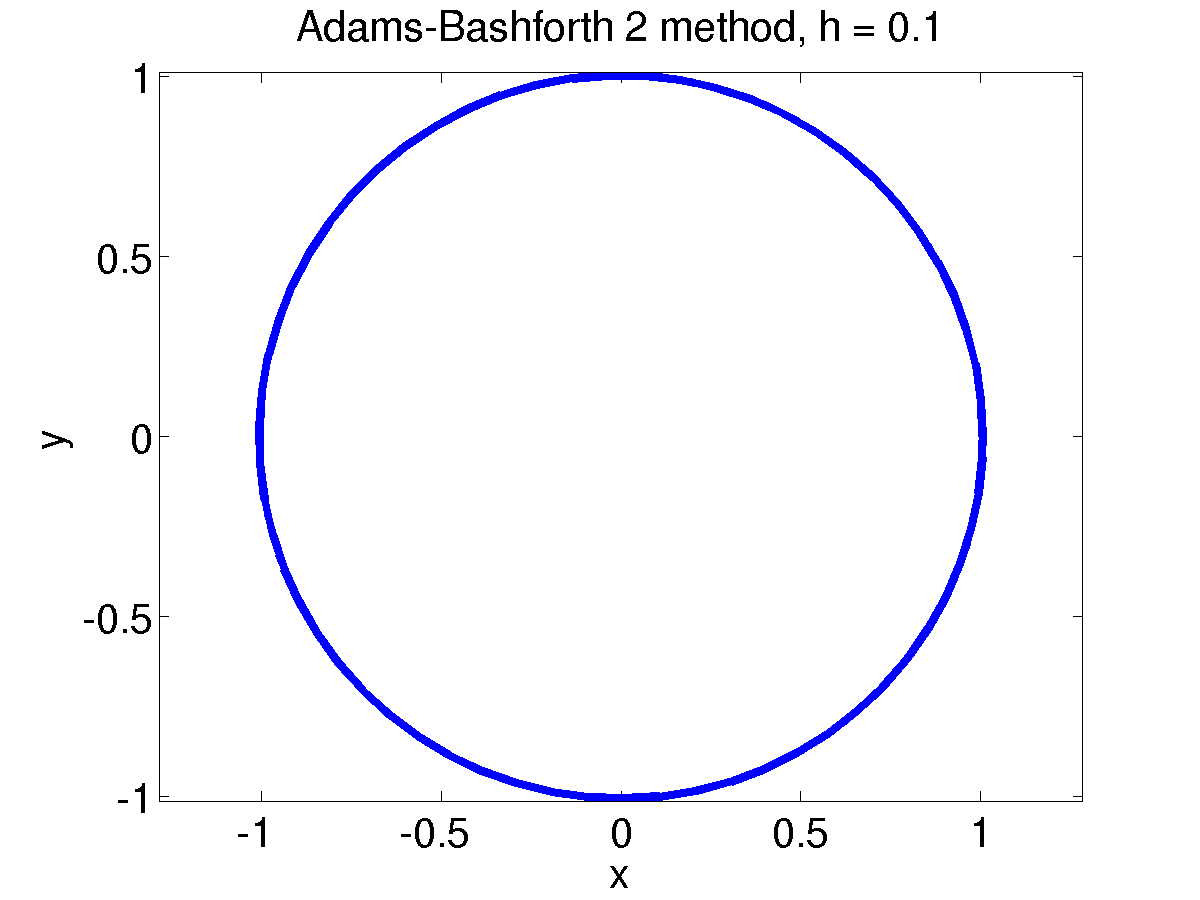
\includegraphics[height=0.5\textheight]{figures/AB2_1}
          \end{center}
        }
        \only<3|handout:1>
        {
          \begin{center}
            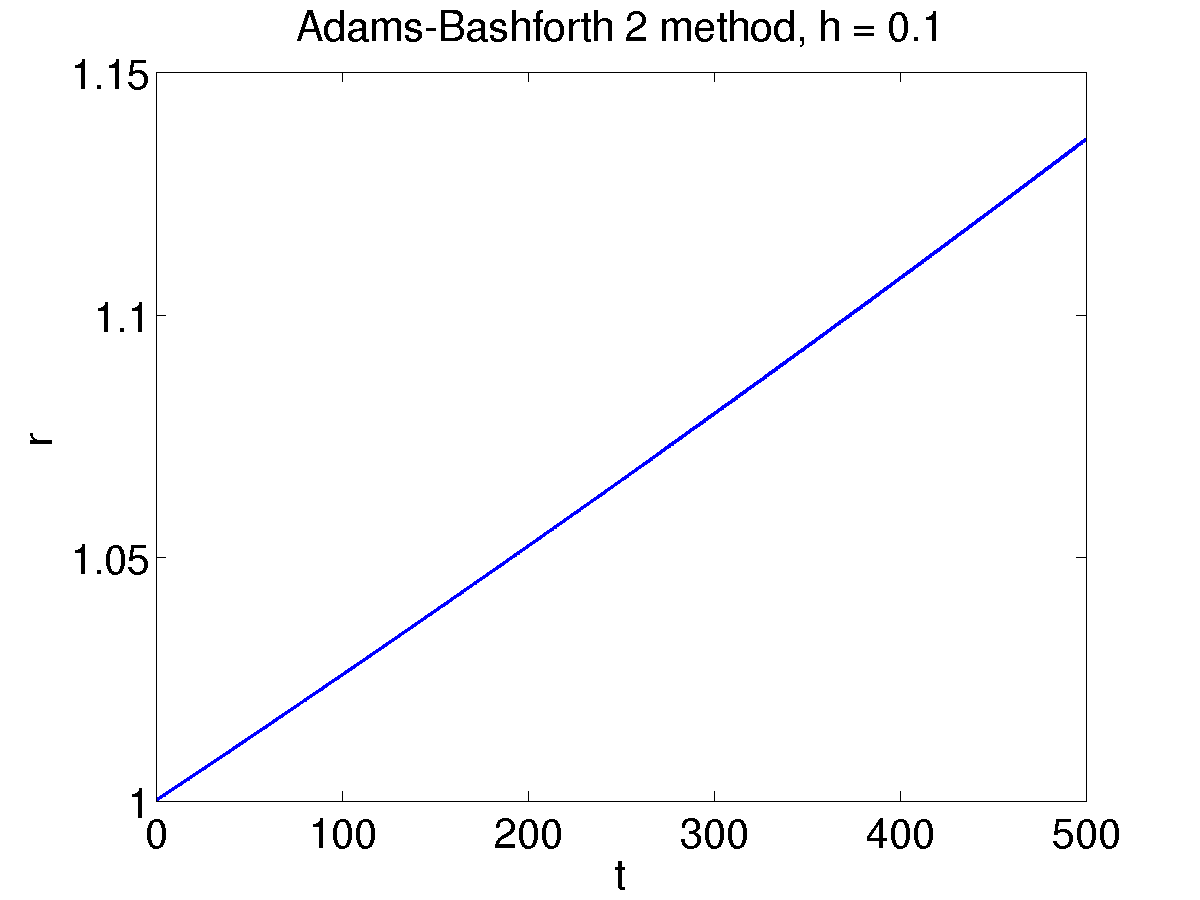
\includegraphics[height=0.5\textheight]{figures/AB2_rad1}
          \end{center}
        }
        \only<4|handout:0>
        {
          \begin{center}
            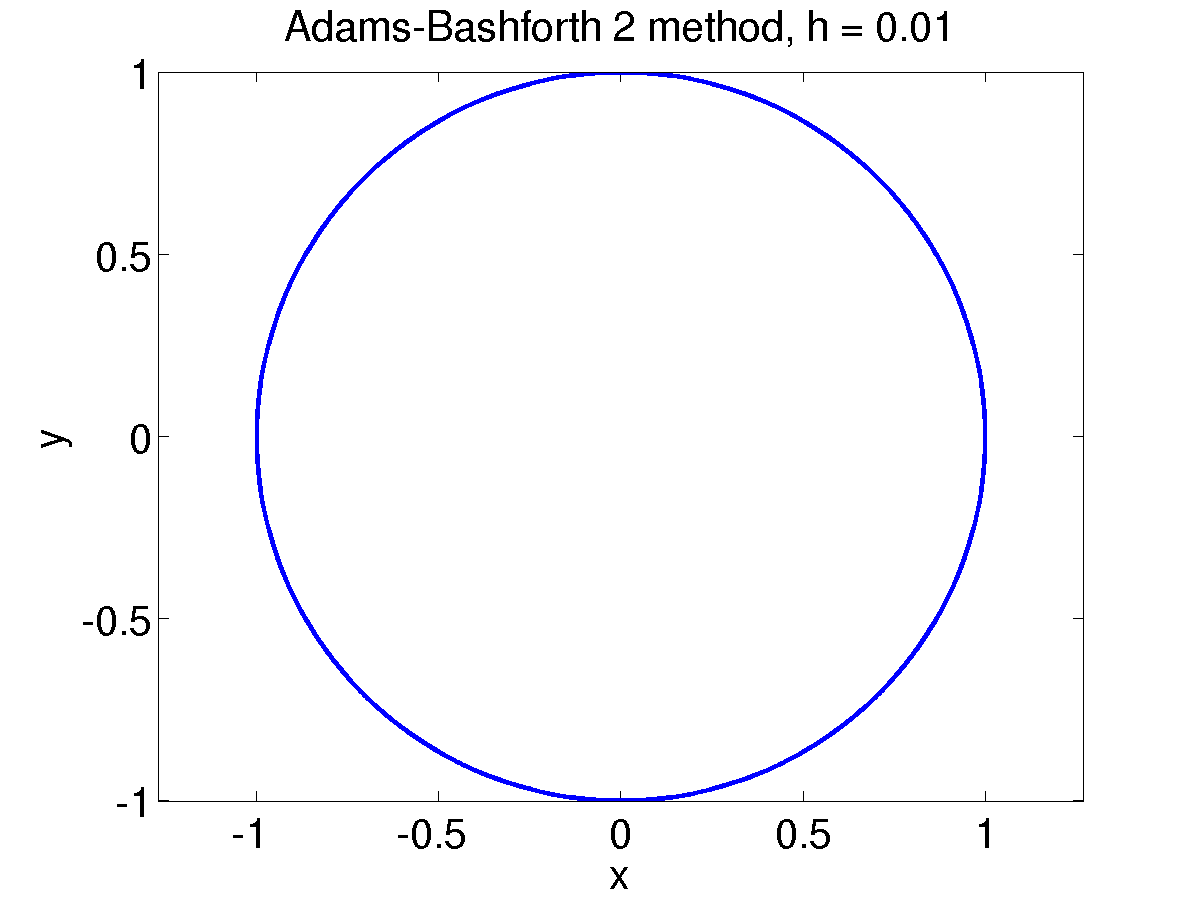
\includegraphics[height=0.5\textheight]{figures/AB2_2}
          \end{center}
        }
        \only<5|handout:2>
        {
          \begin{center}
            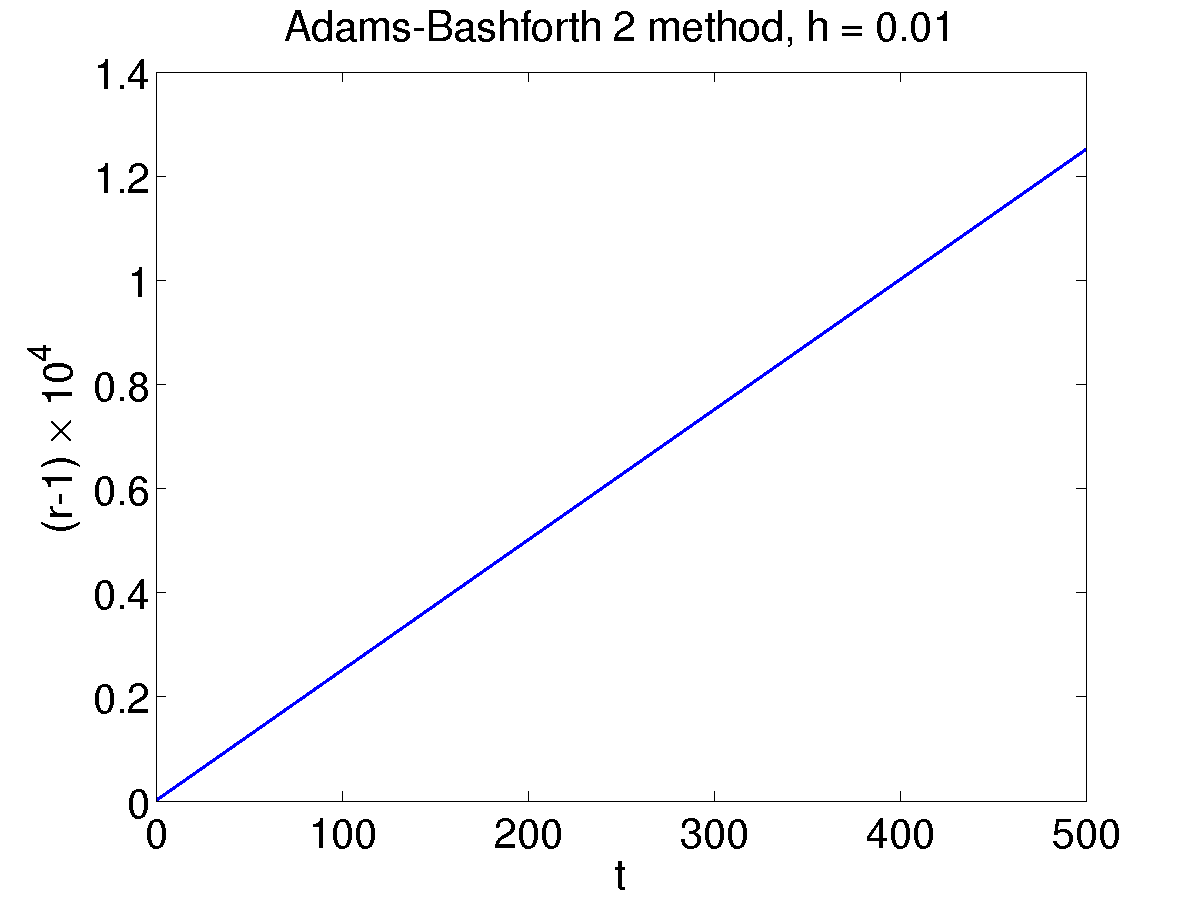
\includegraphics[height=0.5\textheight]{figures/AB2_rad2}
          \end{center}
        }
      \end{overlayarea}
    \end{column}
  \end{columns}

\end{frame}

\begin{frame}
  \frametitle{Higher order Adams-Bashforth}

  Principle behind higher order Adams-Bashforth methods the same;
  solve for the coefficients by integrating
  \begin{equation*}
    y_{n+1} - y_n = h \left[ b_k f_n + b_{k-1} f_{n-1} + \dots b_0
      f_{n + 1 - k} \right]
  \end{equation*}
  over the range, assuming $f(x) = p_s(x)$ for polynomials of degree
  $s = 0, \dots k$. \pause

  \vspace{1ex}

  Easiest to choose as a basis for the polynomials
  \begin{equation*}
    p_{s+1}(x) = x (x + h) \dots (x + h s)
  \end{equation*}
  as $p_{s+1}$ vanishes at $x = 0, -h, \dots, -h s$. \pause Then choose
  $x_n = 0, x_{n - 1} = -h$ and so on: the resulting system of
  equations is in upper-triangular form -- solve by back substitution.

\end{frame}

\begin{frame}
  \frametitle{Higher order Adams-Bashforth example}

  For example, the Adams-Bashforth method of order five has formula
  \begin{equation*}
    y_{n+1} - y_n = h \left[ b_4 f_n + b_3 f_{n-1} + b_2 f_{n-2} + b_1
      f_{n-3} + b_0 f_{n-4} \right] ,
  \end{equation*} \pause
  and the coefficients follow from
  {\small
  \begin{align*}
    p_0 & = 1: & h & = h \left[ b_4 + b_3 + b_2 + b_1 + b_0 \right] \\
    p_1 & = x: & \frac{h^2}{2} & = h \left[ -h \left( b_3 + 2 b_2 + 3
        b_1 + 4 b_0 \right) \right] \\
    p_2 & = x (x + h): & 5 \frac{h^3}{6} & = h \left[ h^2 \left( 2 b_2
        + 6 b_1 + 12 b_0 \right) \right] \\
    p_3 & = x (x + h) (x + 2 h): & 9 \frac{h^4}{4} & = h \left[ -h^3
      \left( 6 b_1 + 24 b_0 \right) \right] \\
    p_4 & = x (x + h) (x + 2 h) (x + 3 h): & 251 \frac{h^5}{30} & = h
    \left[ 24 h^4 b_0 \right].
  \end{align*}
  }
\end{frame}

\begin{frame}
  \frametitle{Standard example}

 Apply the 5 step Adams-Bashforth method to
  \begin{equation*}
    y'(x) = - \sin(x), \quad y(0) = 1
  \end{equation*}
  and integrate to $x = 0.5$. Use RK4 method to start algorithm. Using
  $h = 0.05$ gives
  \begin{center}
    \begin{tabular}{c|c c c c c c}
      $n$ & $x_n$ & $y_n$ & $f(x_n, y_n)$ & $\cos(x_n)$ \\
      \hline
      0 & 0.0 & 1.000 &  0.000 & 1.000 \\
      2 & 0.1 & 0.995 & -0.100 & 0.995 \\
      4 & 0.2 & 0.980 & -0.199 & 0.980 \\
      6 & 0.3 & 0.955 & -0.296 & 0.955 \\
      8 & 0.4 & 0.921 & -0.389 & 0.921 \\
      10 & 0.5 & 0.878 &        & 0.878
    \end{tabular}
  \end{center} \pause
  The error is $3 \times 10^{-6}\%$, not visible at this
  precision. With $h = 0.01$ the error is $2 \times 10^{-9}\%$.
  Convergence is slightly worse than fifth order; result is slightly
  biased by the starting method.

\end{frame}

\begin{frame}
  \frametitle{Standard Example: 2}


  Consider the system
  \begin{equation*}
    \left\{
      \begin{aligned}
        \dot{x} & = -y \\ \dot{y} & = x
      \end{aligned} \right., \quad x(0) = 1, \, \, y(0) = 0.
  \end{equation*}
  In polar coordinates this is $\dot{r} = 0$, $\dot{\phi} = 1$.
  \begin{columns}
    \begin{column}{0.5\textwidth}
      \begin{overlayarea}{\textwidth}{0.4\textheight}
        \only<2-3|handout:1>
        {
          Use the Adams-Bashforth 5 step method with
          $h=0.1$. At $t=500$ the result matches the correct answer to
          the eye.
        }
        \only<3|handout:1>
        {

          \vspace{1ex}
          Looking at the growth of the radius makes the errors
          visible.
        }
        \only<4-5|handout:2>
        {
          Use Adams-Bashforth 5 step method with $h=0.01$. At $t=500$
          the result matches the correct answer to the eye.
        }
        \only<5|handout:2>
        {

          \vspace{1ex}
          Looking at the growth of the radius makes the errors
          visible even now.
        }
      \end{overlayarea}
    \end{column}
    \begin{column}{0.5\textwidth}
      \begin{overlayarea}{\textwidth}{0.6\textheight}
        \only<2|handout:0>
        {
          \begin{center}
            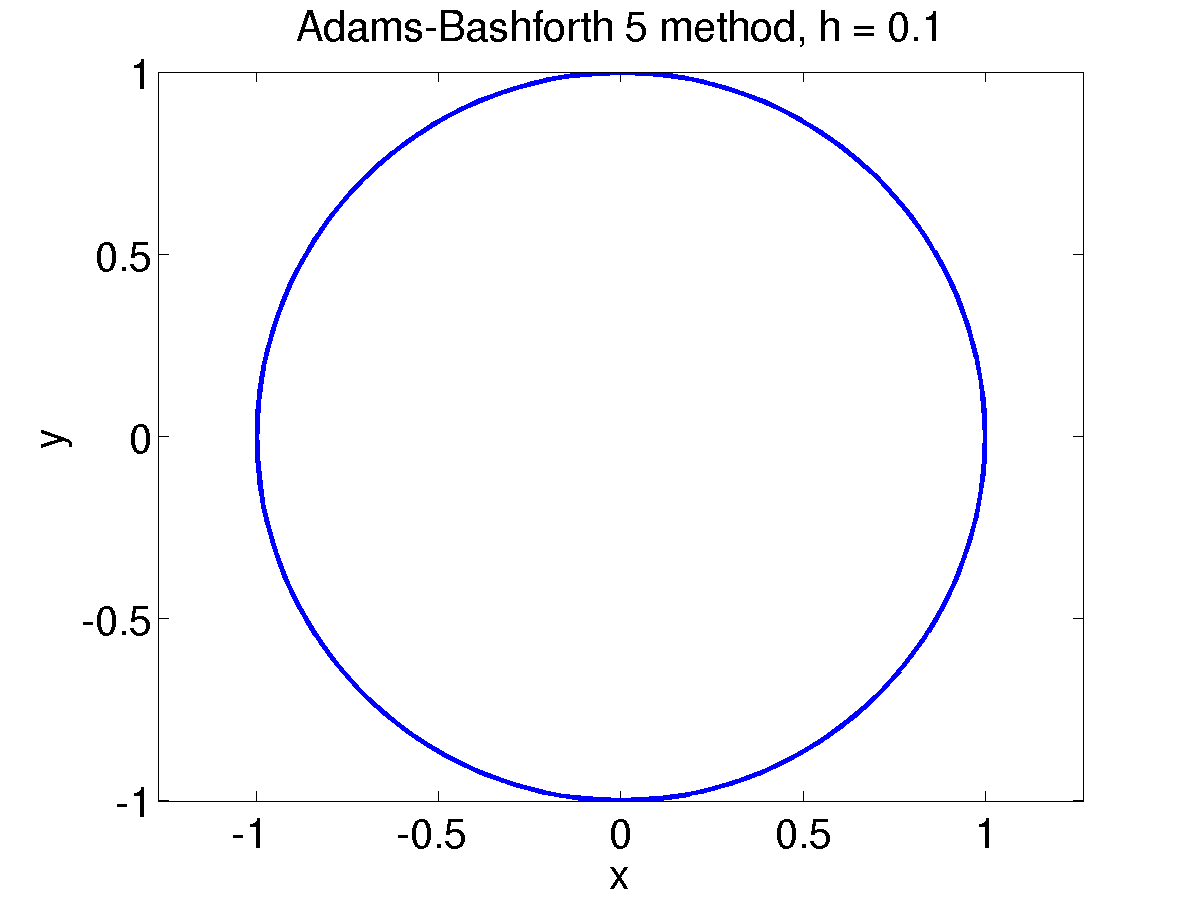
\includegraphics[height=0.5\textheight]{figures/AB5_1}
          \end{center}
        }
        \only<3|handout:1>
        {
          \begin{center}
            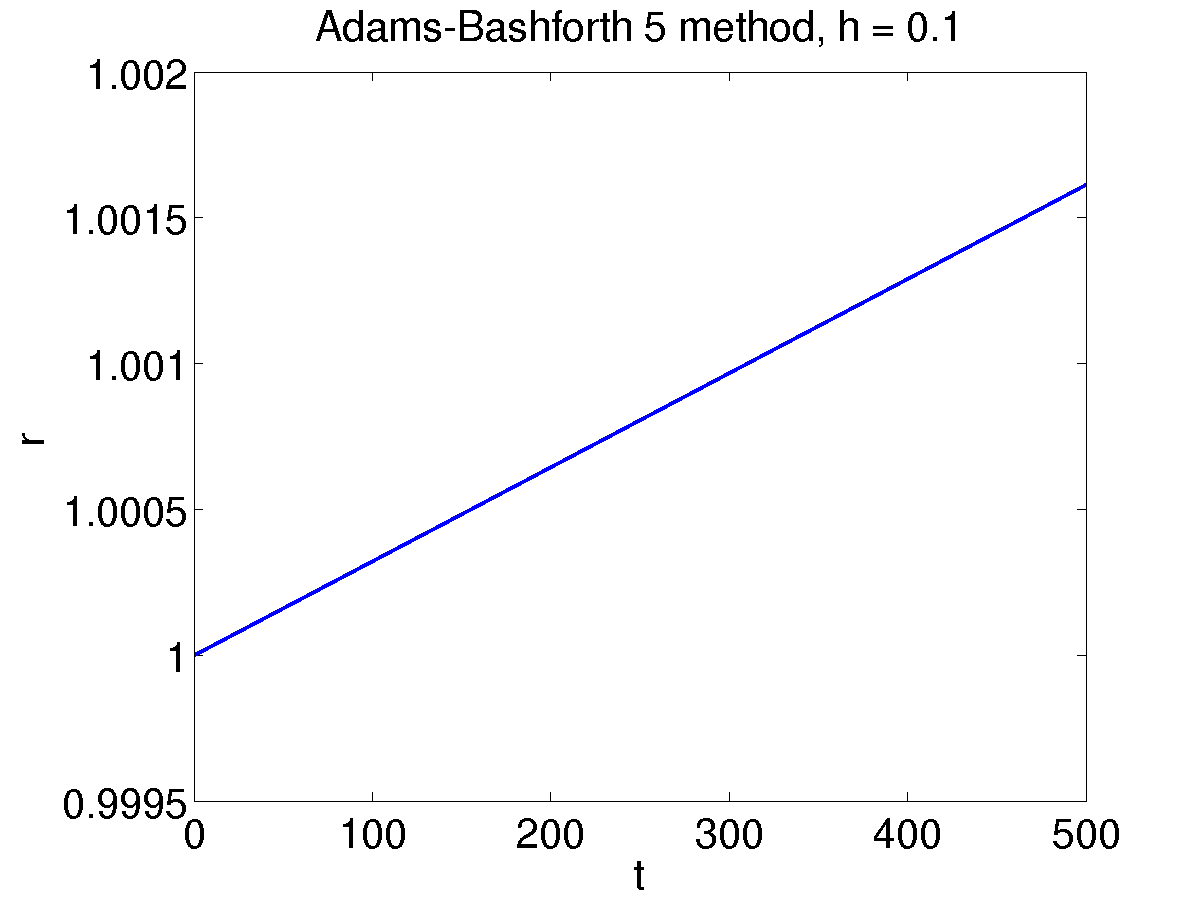
\includegraphics[height=0.5\textheight]{figures/AB5_rad1}
          \end{center}
        }
        \only<4|handout:0>
        {
          \begin{center}
            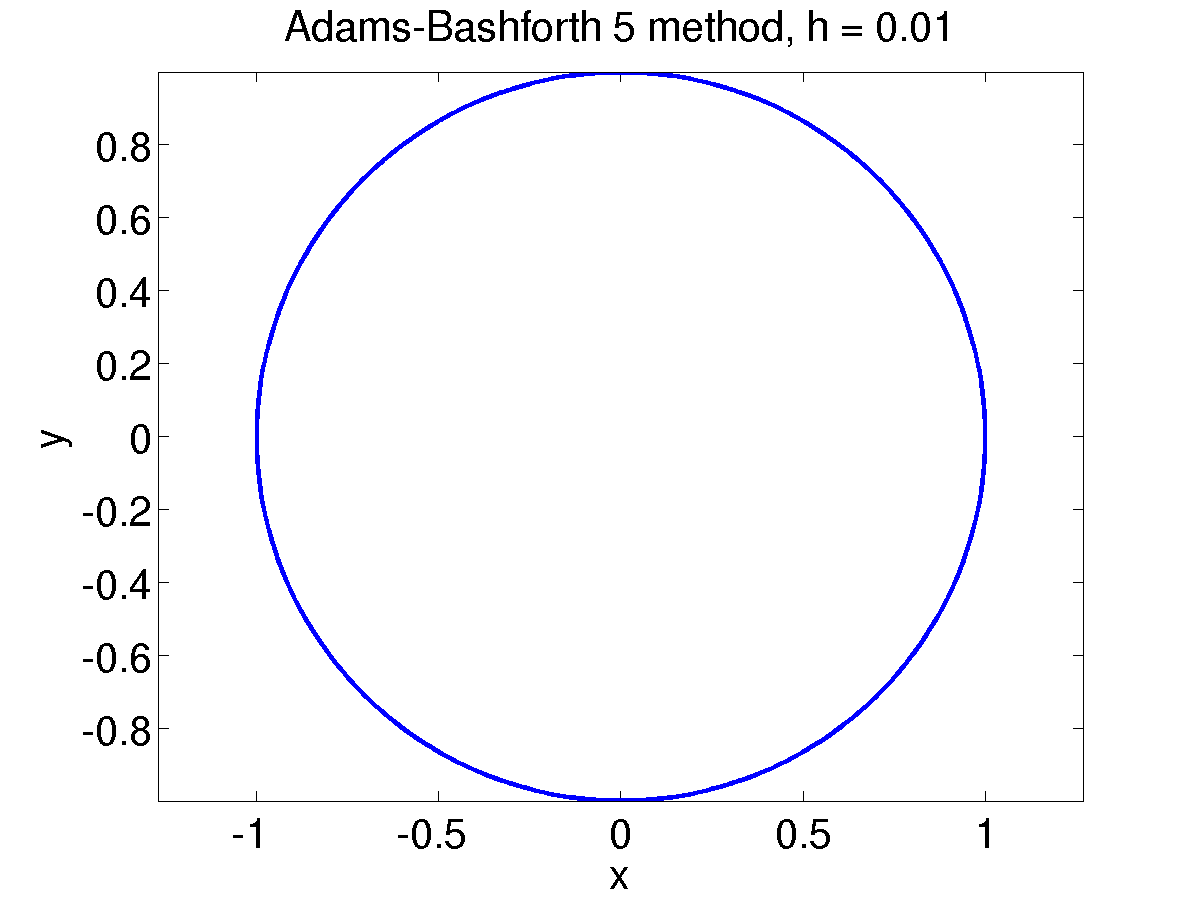
\includegraphics[height=0.5\textheight]{figures/AB5_2}
          \end{center}
        }
        \only<5|handout:2>
        {
          \begin{center}
            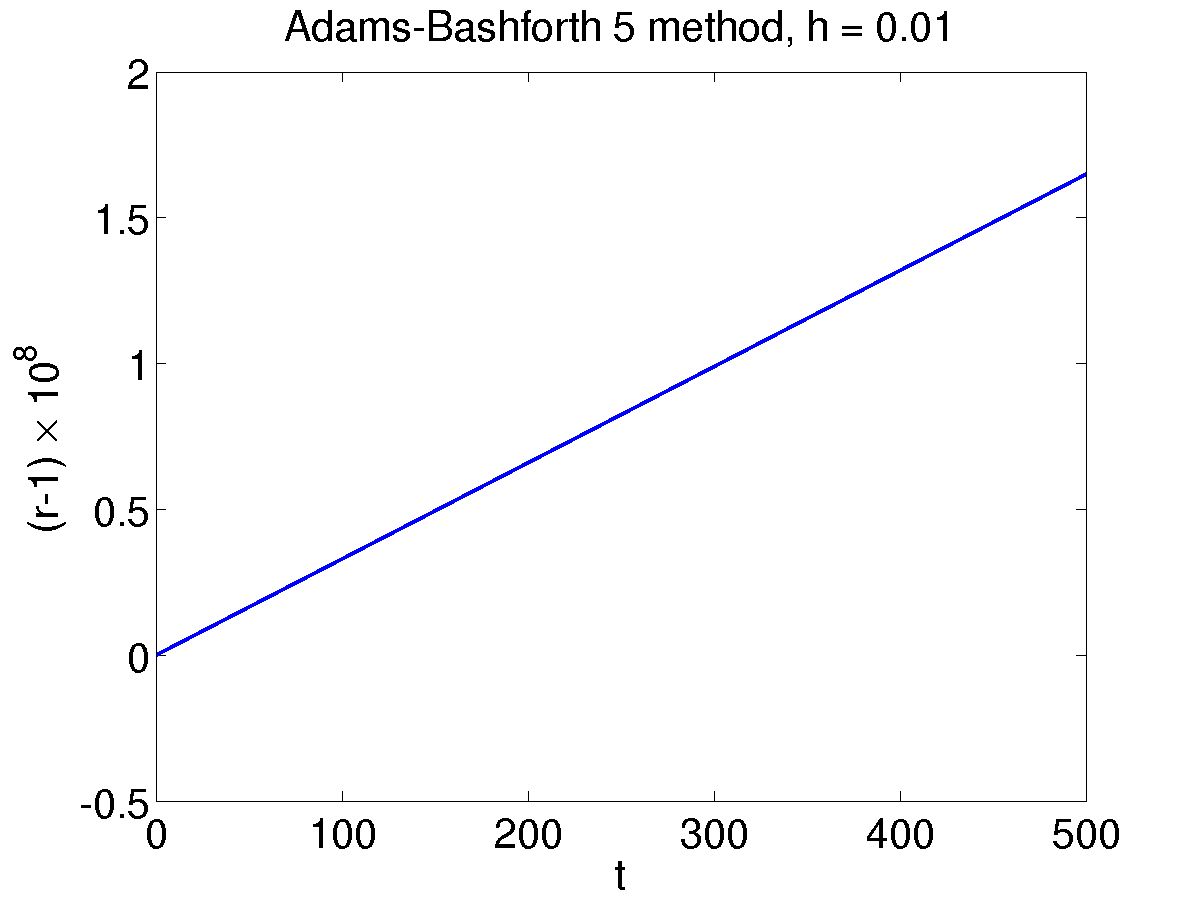
\includegraphics[height=0.5\textheight]{figures/AB5_rad2}
          \end{center}
        }
      \end{overlayarea}
    \end{column}
  \end{columns}

\end{frame}

\section{Summary}

\subsection{Summary}

\begin{frame}
  \frametitle{Summary}

  \begin{itemize}
  \item The Runge-Kutta Fehlberg method, often known as RK45, is a
    fourth order method that estimates its own error using a fifth
    order computation.
  \item When combined with adaptive step sizes this is a standard
    method for solving IVPs to moderate accuracy efficiently. %The Matlab command is {\tt ode45}.
  \item The multistep methods estimate the quadrature solution of the
    IVP, not the derivative.
  \item Multistep methods use a (given) number of prior values of the
    solution at each step.
  \item Multistep methods require fewer function evaluations than
    multistage methods such as Runge-Kutta for the same order of
    accuracy.
  \item It is difficult to use adaptive stepping with multistep
    methods.
  \end{itemize}

\end{frame}

\end{document}



%%% Local Variables:
%%% mode: latex
%%% TeX-master: t
%%% End:
